\documentclass[11pt,a4paper]{article}

\usepackage[margin=1in]{geometry}
\usepackage{amsmath,amssymb,amsthm}
\usepackage{graphicx}
\usepackage{booktabs}
\usepackage{xcolor}
\usepackage[colorlinks=true,linkcolor=blue!60!black,citecolor=blue!60!black,
            urlcolor=blue!60!black]{hyperref}
\usepackage{microtype}
\usepackage{enumitem}

\newtheorem{theorem}{Theorem}
\newtheorem{proposition}[theorem]{Proposition}
\newtheorem{lemma}[theorem]{Lemma}
\theoremstyle{definition}
\newtheorem{definition}[theorem]{Definition}
\theoremstyle{remark}
\newtheorem{remark}[theorem]{Remark}

\newcommand{\C}{\mathbb{C}}
\newcommand{\R}{\mathbb{R}}
\newcommand{\conj}[1]{\overline{#1}}
\newcommand{\lean}[1]{\texttt{\small #1}}

% Boxed callout for retractions and negative results
\usepackage[most]{tcolorbox}
\newtcolorbox{retraction}[1][]{colback=red!3,colframe=red!45!black,
  boxrule=0.5pt,left=4pt,right=4pt,top=3pt,bottom=3pt,#1}
\newtcolorbox{keybox}[1][]{colback=blue!3,colframe=blue!45!black,
  boxrule=0.5pt,left=4pt,right=4pt,top=3pt,bottom=3pt,#1}

\title{\textbf{A dual-scale length for quantum fluids, and a dispersive regulator for a
dyadic shell model:}\\
\large a measurable bound that superfluid $^4$He violates, a Hamiltonian second invariant,
and why the intended measurement could not be made}

\author{Xavier Callens\\
\small SocrateAI-Scientific-QuantumFluids\\
\small \texttt{https://github.com/xaviercallens/SocrateAI-Scientific-QuantumFluids}}

\date{20 September 2026}

\begin{document}
\maketitle

\begin{abstract}
\noindent
Motivated by the T-duality relation $R \leftrightarrow \alpha'/R$, which posits a
self-dual length below which contraction reflects into dilation, we asked whether a
\emph{dispersive} (energy-neutral) small-scale regulator leaves a different signature on a
turbulent cascade than a \emph{dissipative} one. We pose the question in the truncated
dyadic (Katz--Pavlovi\'c) shell model. Three results follow, and one intended result does
not.

First, a structural obstruction: a real-amplitude shell model \emph{cannot} host a
dispersive regulator at all, since every real linear term either damps or forces and
dispersion is phase rotation. We resolve this with a conjugated complexification
$B_n = k_{n-1}a_{n-1}^2 - k_n\conj{a_n}a_{n+1}$ that conserves $\tfrac12\sum|a_n|^2$
exactly while reducing \emph{exactly} to the real model on real data. Second, the
complexification has an unanticipated property: its flow is \emph{volume-preserving}
(Liouville), whereas the real Katz--Pavlovi\'c flow has divergence $-\sum_n k_n a_{n+1}
\neq 0$. Both the conservation law and the shell-local trace identities behind the
Liouville property are machine-checked in Lean 4/Mathlib. Third, the same telescoping
identity that gives conservation yields an exact criterion for a conserving boundary
``bounce'': $\mathrm{Re}(\conj{v_N}^2 v_{N+1}) = 0$, which on real data admits only
truncation but in the complexified model admits $v_{N+1} = i\mu v_N^2$.

The intended measurement---a scaling exponent distinguishing dispersive from dissipative
regularization---was \textbf{not} obtained, and we report why in detail. All three
regulators of the intended comparison are energy-conserving, hence lack an attractor, so
$\sup_t\Omega$ degenerates to the truncation ceiling $k_N^2E$; we identify this as the
known relaxation to \emph{absolute equilibrium} of Galerkin-truncated conservative
systems, established for truncated Euler, truncated Gross--Pitaevskii, and---removing any
novelty claim---for shell models themselves. Seven replacement observables were tried
under pre-registration and all failed. The final diagnosis is methodological and, we
believe, the most transferable output: the model is chaotic, all measurements used single
trajectories, and the fixed-parameter ensemble scatter is $72$--$105\%$ of the mean, far
exceeding the effect sought. Every quantitative and ordinal measurement result in this
work is accordingly retracted, and we state what would be required to obtain one.

Two results added in September 2026 change what the dual-scale idea can be asked to do.
First, the complexified model is \emph{Hamiltonian}: under $w_n = 2^{-n/2}v_n$ it is a
second-harmonic-generation chain, with a second invariant
$H = \sum_n 2^{-n}[\omega_n|v_n|^2 + k_n\,\mathrm{Im}(\conj{v_n}^2 v_{n+1})]$ conserved for
arbitrary real dispersion. Energy conservation is then the Manley--Rowe relation and the
Liouville property is a corollary; $H$ vanishes identically on real data, so the phase is
what carries the second conservation law. A consequence we state as a design rule: a
regulator of order $k^\sigma$ controls the norm of order $k^{\sigma-1}$ uniformly in the
cutoff, so quantum pressure ($\sigma=2$) does \emph{not} reach enstrophy. Second, the
dual-scale shape is made measurable. For a quantum fluid we define the dual length
$\ell(k) = \varepsilon(k)^2/(\hbar^2c^2k^3)$, whose phonon and free-particle limits are
$1/k$ and $k/k_*^2$ with $k_* = 2mc/\hbar$; because the Bogoliubov dispersion is
Pythagorean in those branches, $\ell_B = 1/k + k/k_*^2$ \emph{exactly}, invariant under
$k \mapsto k_*^2/k$ and bounded below by $\sqrt2\,\xi$, with equality at the self-dual
point. On published $^4$He data, with a positive control that first \emph{voided} an
earlier run, the bound fails by a factor $21$ at saturated vapour pressure and $51$ at
$24$~bar. The dual-scale structure is therefore not universal but \emph{localised} to the
weakly interacting regime, and $\ell/(\sqrt2\,\xi)$ is a single dimensionless measure of
the distance from it. No novelty is claimed for the underlying physics.
\end{abstract}

\tableofcontents
\medskip

\begin{keybox}
\textbf{On the character of this report.} This is a mixed positive/negative report. The
analytic and formal results (\S\ref{sec:model}--\ref{sec:seam}) stand and are
machine-checked. The measurement programme (\S\ref{sec:measure}) failed, and its failures
are reported at the same level of detail as the successes, including four retracted
results. Claim identifiers of the form \textsc{claim-nnn} refer to the ledger in the
public repository, where every claim carries its status and, where applicable, its
retraction and reason.
\end{keybox}

\section{Motivation and the question}
\label{sec:intro}

Consider a quantity built from two competing scales, $R + \alpha'/R$. It is invariant
under $R \leftrightarrow \alpha'/R$ and, by the arithmetic--geometric mean inequality,
bounded below by $2\sqrt{\alpha'}$, with equality at the self-dual point
$R = \sqrt{\alpha'}$. We call this shape \emph{dual-scale}. It suggests a class of
small-scale regulators that \emph{reflect} rather than \emph{absorb}: at the self-dual
scale, contraction turns into dilation, and no energy need be removed.

\paragraph{On provenance, stated plainly.} This shape appears in the T-duality relation of
string theory~\cite{GPR1994}, which was the historical motivation for the present work.
\textbf{No string-theoretic content is claimed or used anywhere below}, and an earlier
framing of this programme, which leaned on that language, has been withdrawn. What
survives is arithmetic on two positive terms---and, as \S\ref{sec:duallength} shows, the
fact that the shape occurs \emph{exactly} in a standard dispersion relation, where it
becomes measurable and can therefore be wrong.

Quantum fluids furnish the physical instance in which such a regulator is not
hypothetical. In the Gross--Pitaevskii description, quantum pressure supplies a
small-scale term that is \emph{dispersive}: it rotates phases and conserves energy,
unlike viscosity. The healing length plays the role of the scale below which the
description changes character. The measured phonon--roton dispersion of superfluid
$^4$He~\cite{Godfrin2021,GodfrinKrotscheck2022} is the empirical anchor for that picture.

This suggests a sharp question, which is the one this work set out to answer:

\begin{keybox}
\textbf{Q.} In a turbulent cascade, does a \emph{dispersive} (energy-conserving)
small-scale regulator leave a different signature than a \emph{dissipative} one---or is
only the presence of a cutoff visible, not its mechanism?
\end{keybox}

We pose Q in the truncated dyadic shell model, where the cascade is reduced to a chain of
real amplitudes $a_n$ on wavenumbers $k_n = 2^n$ and blow-up questions are theorems rather
than conjectures~\cite{KatzPavlovic2005}. \S\ref{sec:model}--\ref{sec:seam} construct the
apparatus needed to pose Q there; \S\ref{sec:measure} reports the measurement programme
and its failure; \S\ref{sec:standing} separates what stands from what does not.

\paragraph{Scope, stated once and adhered to.} No claim is made or implied about
Navier--Stokes regularity. No claim is made that Gross--Pitaevskii well-posedness bears on
it. The quantum-pressure analogy fixes the \emph{form} of the regulator studied and
nothing else; in particular the model below is a Bogoliubov-regime construction with no
roton, so the $^4$He dispersion parameters of \S\ref{sec:m1} have no counterpart in it.

\section{The model, and a structural obstruction}
\label{sec:model}

\subsection{The real dyadic model}

With shells $n=0,\dots,N$, wavenumbers $k_n=2^n$, real amplitudes $a_n$, and the
truncation convention $a_{-1}=a_{N+1}=0$, the Katz--Pavlovi\'c/Desnyansky--Novikov model is
\begin{equation}
  \frac{da_n}{dt} \;=\; \underbrace{k_{n-1}a_{n-1}^2 - k_n a_n a_{n+1}}_{B_n(a)}
  \;-\; \nu k_n^2 a_n ,
  \qquad
  E = \tfrac12\textstyle\sum_n a_n^2, \quad
  \Omega = \tfrac12\textstyle\sum_n k_n^2 a_n^2 .
  \label{eq:real}
\end{equation}
The nonlinearity conserves $E$ exactly under truncation.

\subsection{The obstruction}

\begin{proposition}[No dispersive regulator exists in a real-amplitude model]
\label{prop:obstruction}
Let $-c(k_n)a_n$ be any linear regulator with $c$ real. Its contribution to the energy is
$\frac{d}{dt}\big(\tfrac12\sum a_n^2\big) \supset -\sum_n c(k_n)a_n^2$, which is
$\le 0$ if $c\ge0$ and $\ge 0$ if $c\le0$. \emph{No} real linear regulator is
energy-neutral.
\end{proposition}

Energy-neutrality is precisely what distinguishes dispersion from dissipation. The
obstruction is therefore structural, not a shortage of ingenuity: dispersion is phase
rotation, and a real amplitude has no phase to rotate. Answering Q requires enlarging the
state space---a change of \emph{model}, not of regulator.

\subsection{A complexification that is not the obvious one}

The naive complexification (keep~\eqref{eq:real}, let $a_n\in\C$) fails: measured over
$200$ random complex states at $N=10$, $\max|dE/dt| = 8.7\times10^3$. Placing a single
conjugation on the \emph{outgoing} term repairs it:
\begin{equation}
  \boxed{\;B_n(v) \;=\; k_{n-1}v_{n-1}^2 \;-\; k_n\,\conj{v_n}\,v_{n+1}\;}
  \label{eq:conj}
\end{equation}

\begin{theorem}[Exact conservation; \lean{shellBc\_energy\_conservation}]
\label{thm:conservation}
With $v_{N+1}=0$, $\;\sum_{n\le N}\mathrm{Re}\big(\conj{v_n}B_n(v)\big) = 0$.
\end{theorem}

\begin{proof}[Proof sketch]
The pairing telescopes. Writing $\mathrm{out}_m = k_m\,\mathrm{Re}(\conj{v_m}^2v_{m+1})$,
one shows $\sum_{n\le N}\mathrm{Re}(\conj{v_n}B_n) = -\mathrm{out}_N$ by induction, the
cancellation at each step being the identity
$\mathrm{Re}(\conj{a}^2b) = \mathrm{Re}(a^2\conj{b})$---both sides are the real part of a
conjugate pair. Setting $v_{N+1}=0$ gives the result. Machine-checked; see
\S\ref{sec:formal}.
\end{proof}

Three consequences deserve statement.

\begin{proposition}[Exact reduction; the reals are invariant]
\label{prop:real}
On real data $\conj{v_n}=v_n$, so~\eqref{eq:conj} coincides \emph{identically}
with~\eqref{eq:real}, and $\mathrm{Im}\,B_n = 0$. Every solution of the real model---%
including the finite-time blow-up solutions of the inviscid infinite system~%
\cite{KatzPavlovic2005}---remains a solution.
\end{proposition}

This is what makes the complexification an extension rather than a replacement, and it
supplies a stringent validation (\S\ref{sec:posctl}). It is also why the choice is not
merely aesthetic: other conjugation placements also conserve energy, and this one is
selected for Proposition~\ref{prop:real}. \textbf{The complexification is a labelled
deformation, not a derivation.}

\subsection{The two regulators}

With complex amplitudes, dissipation and dispersion become the same $k^2$ term with the
coefficient rotated by ninety degrees in $\C$:
\begin{equation}
  \underbrace{-\nu k_n^2 v_n}_{\text{dissipative},\ \nu\in\R}
  \qquad\text{versus}\qquad
  \underbrace{-\,i D k_n^2 v_n}_{\text{dispersive},\ D\in\R}
  \label{eq:regs}
\end{equation}
Measured energy rates: the viscous term drives $dE/dt$ strictly negative; the dispersive
term is neutral to $\max|dE/dt| = 2.7\times10^{-11}$. Because the two share their
$k$-dependence exactly and differ only in the phase of the coefficient, the comparison
isolates \emph{dispersive versus dissipative} without confounding it with a different
spectral slope. In the Gross--Pitaevskii reading $D = \hbar/2m$, and the crossover between
the phonon branch $\omega\approx ck$ and the free branch $\omega\approx Dk^2$ sits at the
healing length $\xi = D/c$.

\section{Liouville structure}
\label{sec:liouville}

The complexification has a property we did not anticipate and that changes the character
of the model.

\begin{theorem}[Volume preservation; \lean{shell\_divergence\_zero}]
\label{thm:liouville}
Regard $\C^{N+1}\cong\R^{2N+2}$. The diagonal blocks of the derivative of the complexified
flow have zero real trace: for every $w\in\C$ the $\R$-linear map $v\mapsto \conj{v}w$ has
zero trace, and multiplication by a purely imaginary constant has zero trace. Hence the
flow of~\eqref{eq:conj} together with~\eqref{eq:regs} at $\nu=0$ is divergence-free.
\end{theorem}

The real model is \emph{not}: its divergence is $-\sum_n k_n a_{n+1}$, verified numerically
against the analytic formula to four decimals. Figure~\ref{fig:liouville} shows the
dichotomy directly.

\begin{figure}[t]
\centering
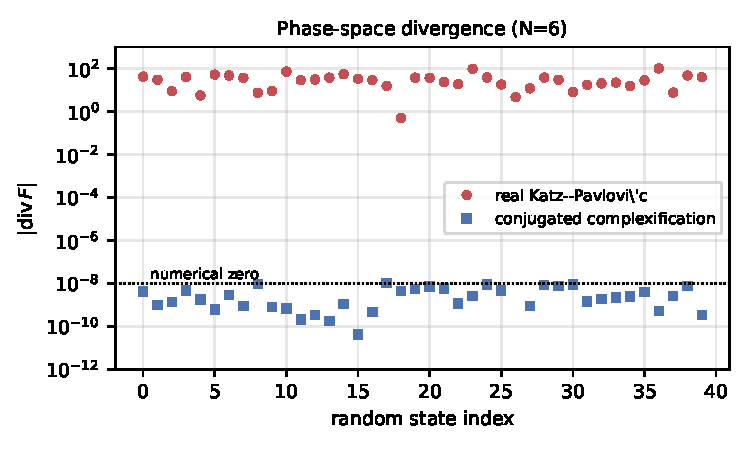
\includegraphics[width=0.62\textwidth]{figures/liouville.pdf}
\caption{Phase-space divergence over random states. The conjugated complexified flow is
divergence-free to round-off ($\sim10^{-9}$); the real Katz--Pavlovi\'c flow is not, with
$|\mathrm{div}\,F|$ of order $10$--$10^2$. Volume preservation is what licenses the
statistical-equilibrium description of \S\ref{sec:degeneracy}.}
\label{fig:liouville}
\end{figure}

\begin{remark}[Interpretation, flagged as such]
Volume preservation on the compact energy sphere gives Poincar\'e recurrence and makes
equilibrium statistical mechanics applicable. It is suggestive that the real dyadic model,
whose literature concerns blow-up and regularity, is volume-contracting along cascade
states, while the complexification lands in the Liouville class where the shell-model
\emph{statistical equilibrium} literature operates~\cite{Aurell1994,Ditlevsen1996,%
Thalabard2016,TomRay2017}. We record the observation and claim nothing further from it.
\end{remark}

\section{The boundary seam: a conserving ``bounce''}
\label{sec:seam}

The T-duality motivation suggests a reflecting seam at the cutoff rather than truncation.
The telescoping identity of Theorem~\ref{thm:conservation} settles exactly which seams are
admissible.

\begin{proposition}[Conserving-seam criterion]
\label{prop:seam}
A boundary condition $v_{N+1}=g(v)$ conserves energy if and only if
$\mathrm{Re}\big(\conj{v_N}^2\,v_{N+1}\big) = 0$, i.e.\ iff $v_{N+1}\perp v_N^2$ under the
real inner product $\mathrm{Re}(\conj{x}y)$.
\end{proposition}

Two corollaries follow, and they cut in opposite directions:
\begin{itemize}[leftmargin=1.4em,itemsep=1pt]
  \item \textbf{On real data, truncation is the only conserving seam.} The criterion
  reduces to $v_N^2 v_{N+1}=0$. A reflective seam $v_{N+1}=v_{N-1}$ \emph{leaks}, so a
  ``bounce'' built that way would measure broken conservation rather than the bounce.
  \item \textbf{In the complexified model a conserving family exists:}
  $v_{N+1} = i\mu v_N^2$ gives $\conj{v_N}^2(i\mu v_N^2) = i\mu|v_N|^4$, purely imaginary.
  There is \emph{no real analogue}. Substituting into shell $N$'s outgoing term yields
  $-i\mu k_N |v_N|^2 v_N$: a cubic self-phase-modulation term, i.e.\ an NLS/GPE-type
  nonlinearity localized at the cutoff.
\end{itemize}

That the only energy-conserving bounce available is GPE-like is a pleasing coincidence and
is treated as no more than that; the content here is the algebra.

\section{Formalization}
\label{sec:formal}

Theorems~\ref{thm:conservation}, \ref{thm:liouville} and
Propositions~\ref{prop:real}, \ref{prop:seam} (both directions) are machine-checked in
Lean~4 against Mathlib~\cite{Mathlib}, deliberately mirroring the real-model development of
the sibling stream so the two compare line by line and pinning the same library revision.

\begin{center}
\small
\begin{tabular}{@{}lll@{}}
\toprule
Lean name & Content & Axioms \\
\midrule
\lean{re\_conj\_sq\_mul} & $\mathrm{Re}(\conj{a}^2b)=\mathrm{Re}(a^2\conj{b})$ & standard \\
\lean{sum\_re\_conj\_mul\_shellBc} & telescoping identity & standard \\
\lean{shellBc\_energy\_conservation} & Theorem~\ref{thm:conservation} & standard \\
\lean{shellBc\_real} & Proposition~\ref{prop:real} (invariance) & standard \\
\lean{rtrace\_mulRight} & $\mathrm{tr}_\R(\cdot\,c) = 2\,\mathrm{Re}\,c$ & standard \\
\lean{rtrace\_mul\_I} & imaginary multiplier: zero trace & standard \\
\lean{rtrace\_conj\_mul} & $v\mapsto\conj{v}w$: zero trace & standard \\
\lean{shell\_divergence\_zero} & Theorem~\ref{thm:liouville} (shell block) & standard \\
\lean{seam\_conserves\_iff} & Proposition~\ref{prop:seam}, both directions & standard \\
\lean{seam\_zero\_conserves} & truncation conserves (corollary) & standard \\
\lean{seam\_gpe\_conserves} & $v_{N+1}=i\mu v_N^2$ conserves (corollary) & standard \\
\bottomrule
\end{tabular}
\end{center}

\noindent
``Standard'' denotes the axiom set \texttt{[propext, Classical.choice, Quot.sound]} and
in particular the absence of \texttt{sorryAx}. The repository's verification gate builds
the development and fails on either a build error or a \texttt{sorryAx} in any certificate;
the gate was itself negative-controlled by inserting a \texttt{sorry} and confirming
detection.

\subsection{Validation against an independent implementation}
\label{sec:posctl}

Proposition~\ref{prop:real} supplies an unusually stringent check: at $D=0$ with real
initial data the complexified model must reproduce an independent implementation of the
\emph{real} model exactly. Against the sibling stream's implementation (written separately,
in a different style) the agreement is bit-for-bit---relative difference $0.00\mathrm{e}{+}00$
on all nine tested configurations, for both the peak enstrophy and the final energy, across
$\sim\!2.4\times10^6$ RK4 steps.

The exactness was checked rather than assumed: $k_n=2^n$ are exact powers of two, so
multiplication by them shifts the IEEE-754 exponent without touching the mantissa, and the
two implementations' differently-associated products therefore agree bit-for-bit. For a
generic $k$ they would differ at $\sim10^{-14}$; a shell model with spacing $\lambda\neq2$
would require a tolerance here rather than an equality.

\paragraph{What is and is not formalized.} The trace identities are proved. Their
\emph{assembly} into the statement ``these are the diagonal blocks of the flow
derivative'' is by inspection of the definition and is verified numerically, not formally.
We state the boundary rather than let the presence of Lean imply more coverage than exists.

\section{Empirical anchor: reproducing the $^4$He dispersion}
\label{sec:m1}

As an instrument calibration, we reproduced the Landau parameters from the published
dispersion table of Godfrin et al.~\cite{Godfrin2021} (1727 points at $P=0$, distributed
as an ancillary file with the preprint). Fitting a linear phonon branch and a parabolic
roton branch gives $c = 1.5716\pm0.0003\;\mathrm{meV\,\AA}$ and
$\Delta = 0.7442\pm0.0005$~meV, agreeing with six independently attributed determinations
to within $0.20\%$ and $0.03$--$0.33\%$ respectively---against tolerances of $5\%$ and
$10\%$.

\begin{remark}[Two honest caveats]
(i) The reference values initially used in this work were misattributed: values recalled
from memory were credited to Cowley--Woods (1971) and Glyde et al.\ (1998), neither of
which reports the Landau triple---the latter measures $2.0\le Q\le 4.0$~\AA$^{-1}$,
entirely beyond the roton, and so cannot report a sound velocity at all. The comparison
above uses corrected, source-traced values. (ii) Godfrin et al.'s own $P=0$ roton gap is
itself calibrated to an earlier determination, so extracting $\Delta$ from their curve is
partly circular; what the fit legitimately demonstrates is that the pipeline
\emph{recovers} the parameter encoded in the curve.
\end{remark}

\section{The measurement programme, and why it failed}
\label{sec:measure}

\subsection{All three intended regulators are conservative}
\label{sec:degeneracy}

The intended comparison used three regulators: truncation (control), a T-dual ``bounce'',
and the dispersive term. \emph{All three conserve energy}---truncation exactly
($v_{N+1}=0$ kills the outflux), the dispersive term by construction, the bounce only for
the seams of Proposition~\ref{prop:seam}. None dissipates. Consequently none has an
attractor, and $\sup_t\Omega$ does not settle: it climbs toward the ceiling $k_N^2E$, a
property of the \emph{truncation} rather than of the regulator (Figure~\ref{fig:degeneracy}).

\begin{figure}[t]
\centering
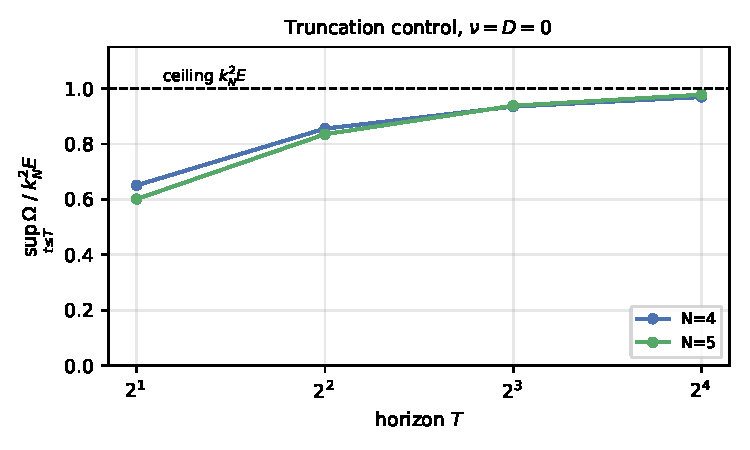
\includegraphics[width=0.62\textwidth]{figures/degeneracy.pdf}
\caption{$\sup_{t\le T}\Omega$ for the truncation control at $\nu=D=0$, normalized by the
energy-conservation ceiling $k_N^2E$. The observable climbs toward the ceiling at each $N$,
so its exponent against $\alpha'=4^{-N}$ tends to $-1$: the trivial bound restated,
carrying no dynamical information.}
\label{fig:degeneracy}
\end{figure}

\begin{keybox}
\textbf{This is a known phenomenon, and we claim no novelty.} Relaxation of
Galerkin-truncated conservative systems toward \emph{absolute equilibrium} was introduced
by Lee~\cite{Lee1952} and Kraichnan~\cite{Kraichnan1973}, demonstrated for truncated Euler
by Cichowlas et al.~\cite{Cichowlas2005} (whose transient behaves dissipatively), and for
the truncated Gross--Pitaevskii/NLS family by Davis et al.~\cite{Davis2001},
Connaughton et al.~\cite{Connaughton2005} and Krstulovic--Brachet~\cite{Krstulovic2011}.
Decisively for novelty, statistical equilibrium in \emph{shell models} is established
territory~\cite{Aurell1994,Ditlevsen1996,TomRay2017}, most directly by
Thalabard--Turkington~\cite{Thalabard2016} (``relaxation \dots{} towards Gibbs equilibrium
in an inviscid shell model''). Our observation is a re-expression in a dyadic variant, not
a new phenomenon. We found no prior thermalization study of the Katz--Pavlovi\'c model
specifically, whose literature concerns blow-up.
\end{keybox}

Notably, Krstulovic--Brachet~\cite{Krstulovic2011} report a \emph{dispersive bottleneck
delaying thermalization} in the truncated GPE---which is precisely the hypothesis our
measurement then set out to test in this model, with a named precedent rather than as a
speculation.

\subsection{Seven observables, under pre-registration}

Since $\sup_t\Omega$ degenerates, we sought a replacement, adopting a pre-registered
validation battery whose criteria were fixed before each run and which grew as each
failure exposed a missing check. Seven candidates were tested:

\begin{center}
\small
\begin{tabular}{@{}llp{7.6cm}@{}}
\toprule
Observable & Family & Outcome \\
\midrule
$\sup_t\Omega$ & amplitude & horizon-degenerate (Fig.~\ref{fig:degeneracy}) \\
time-averaged $\Omega$ & amplitude & decays as $1/T$ for the dissipative arm \\
$\max_t d\Omega/dt$ & amplitude & horizon-dependent, $19\%$ drift \\
$\Omega$ at first peak & amplitude & non-monotonic: new local maxima appear as $D$ falls \\
$\max_{t\le T^*}\Omega$ & amplitude & $\beta$ drifts $40\%$ with its own window $T^*$ \\
$t_{\text{peak}}$ & timescale & no power law on the dispersive arm ($r^2=0.24$) \\
$\tau_f$ (crossing time) & timescale & fitted exponent failed the battery; see below \\
\bottomrule
\end{tabular}
\end{center}

\subsection{The diagnosis: single trajectories of a chaotic system}

\begin{retraction}
\textbf{Retraction.} Every quantitative and ordinal measurement result in this programme is
withdrawn. The exponents fitted to $\tau_f$ and to the excess delay
$\tau-\tau_0$ failed their own pre-registered criteria; an apparent ordinal result
(``stronger dispersion delays thermalization, censoring perfectly ordered'') was a
single-sample artifact; and an apparent sign reversal at small $D$ was noise.
\end{retraction}

The final diagnosis subsumes the individual failures. The model is chaotic and every
measurement used \emph{one} trajectory. Fixing all physical parameters and varying only
the initial phases---identical $|a_n|$, identical energy---the thermalization time scatters
by $72$--$105\%$ of its mean (Figure~\ref{fig:scatter}). At $D=0.05$, half the
realizations failed to reach the level while the rest reached it. The effect sought was
$2$--$20\%$.

\begin{figure}[t]
\centering
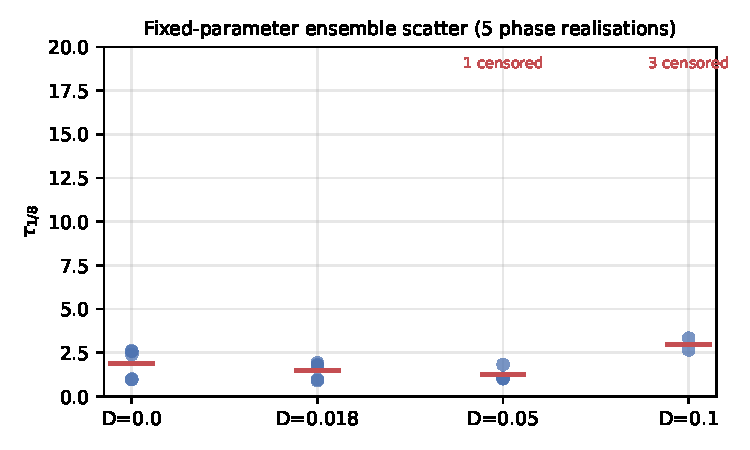
\includegraphics[width=0.62\textwidth]{figures/scatter.pdf}
\caption{Thermalization time $\tau_{1/8}$ across five phase realizations at fixed
parameters (identical $|a_n|$, identical energy); red dashes mark ensemble means. Scatter
is comparable to the mean, and at $D=0.05$ half the realizations are censored. All
measurements in this programme used a single realization.}
\label{fig:scatter}
\end{figure}

\begin{keybox}
\textbf{Why the battery missed it.} All six criteria tested \emph{deterministic}
reproducibility---the same trajectory at finer timestep or finer sampling, or a
neighbouring parameter on the same trajectory family. \textbf{None tested statistical
reproducibility across trajectories drawn from the same physical ensemble.} In a chaotic
system that is the binding constraint. Timestep refinement passing at $0.00\%$ on all
twelve points of one round was silent about it: it is the wrong limit.
\end{keybox}

This also replaces ``seven observables, six failure modes'' with a single cause: the
non-monotonicity, own-parameter drift and cross-level instabilities are all consistent with
single-trajectory sampling. (Horizon degeneracy is genuinely separate---that concerns the
ceiling, not sampling.) And it explains a false corroboration: the apparent small-$D$ sign
reversal appeared in all four level/convention combinations, which read as mutual
confirmation but was not, since those sub-analyses shared a trajectory.
\emph{Consistency across sub-analyses is not evidence when they share a source of noise.}

\subsection{What a real measurement would require}

Not another observable. Ensemble measurement: with coefficient of variation $23$--$49\%$,
a $5\%$ determination of the mean needs $n\approx22$--$97$ realizations \emph{per
parameter point}---one to two orders of magnitude more computation than was expended---%
fitting ensemble means rather than single trajectories, with the ensemble-scatter check
performed \emph{first} to size the campaign. Whether an exponent then exists is open; all
that is currently established is that the effect, if real, lies below the resolution of
what was spent.

\section{A Hamiltonian second invariant, and what a dispersive regulator buys}
\label{sec:hamiltonian}

The obstruction of \S\ref{sec:measure} is that every regulator considered conserves energy,
so the truncated system thermalizes and amplitude observables measure the cutoff. That
raises a structural question the measurement programme never reached: \emph{is
conservation all there is}, or does the complexified model carry more?

\paragraph{Riding the graded phase.} The uniform phase rotation $v_n \mapsto e^{i\theta}v_n$
is \emph{not} a symmetry of the flow, since $v_{n-1}^2$ acquires $e^{2i\theta}$. The
\emph{graded} rotation $v_n \mapsto e^{i2^n\theta}v_n$ is: both $k_{n-1}v_{n-1}^2$ and
$k_n\conj{v_n}v_{n+1}$ carry charge $2^n$. A continuous symmetry suggests a Hamiltonian
structure, and the rescaling $w_n = 2^{-n/2}v_n$ exhibits one: in those variables the model
is a chain of second-harmonic generators, two quanta of shell $n$ fusing into one of shell
$n+1$.

\begin{theorem}[Second invariant]
\label{thm:second}
For weights satisfying $g_{n+1}\,(2k_n) = g_n\,k_{n+1}$---for instance $g_n = 2^{-n}k_n$---the
functional
\[
   H(v) \;=\; \sum_n g_n\,\mathrm{Im}\!\left(\conj{v_n}^2 v_{n+1}\right)
\]
is conserved by the truncated flow. With a dispersive term $-i\omega_n v_n$ the conserved
functional is $H = \sum_n 2^{-n}\bigl[\omega_n|v_n|^2 + k_n\,\mathrm{Im}(\conj{v_n}^2
v_{n+1})\bigr]$, for \emph{arbitrary} real $\omega_n$, and the conserving seam
$v_{N+1} = i\mu v_N^2$ adds $\tfrac12\mu k_N 2^{-N}|v_N|^4$.
\end{theorem}

The telescoping identity and the vanishing of the rate under truncation are machine-checked
(\lean{ShellHamiltonian.lean}, axiom footprint $\{$\lean{propext}, \lean{Classical.choice},
\lean{Quot.sound}$\}$); a control with the factor $2$ removed fails to compile. The
dispersive and seam extensions are verified as exact polynomial identities in computer
algebra for general $k_n$, $\omega_n$, $\mu$, not in Lean.

Three consequences follow, and they reorganise \S\ref{sec:liouville}:
\begin{enumerate}\itemsep2pt
\item the Liouville property (Thm.~\ref{thm:liouville}) is a \emph{corollary} of Hamiltonian
      structure, not an independent fact;
\item exact energy conservation (Thm.~\ref{thm:conservation}) is the Manley--Rowe relation,
      the Noether charge of the graded phase;
\item $H \equiv 0$ identically on real data. \emph{The phase is what carries the second
      conservation law}, which is the precise sense in which the complexification is not
      cosmetic.
\end{enumerate}

\paragraph{The $\sigma$-rule.} Bounding the cubic term by $\sqrt{S}\,S$ with
$S = \sum|v_n|^2$ gives, uniformly in the cutoff,
\[
   \textstyle\sum_n 2^{-n}\omega_n |v_n|^2 \;\le\; H + (2E)^{3/2},
\]
also machine-checked. Reading $\omega_n = D k_n^\sigma$ with $k_n = 2^n$: \emph{a dispersive
regulator of order $k^\sigma$ controls the norm of order $k^{\sigma-1}$, uniformly in the
truncation}. Quantum pressure has $\sigma = 2$ and therefore controls $\sum k_n|v_n|^2$ and
\textbf{not} the enstrophy $\sum k_n^2|v_n|^2$; reaching enstrophy would require
$\sigma = 3$. This is the sharpest available answer to the question of \S\ref{sec:intro}:
the dispersive regulator does buy something uniform in the cutoff, but one power of $k$ less
than the quantity the measurement programme was built around.

\paragraph{What is \emph{not} there.} A deterministic search over all quadratic and quartic
functionals ($N \le 6$, both seams, with a positive control backed by the truncated
Gross--Pitaevskii energy and a negative control on a leaking seam) finds the nullspace to be
exactly $\{$mass, mass$^2$, $H\}$ and \emph{no} invariant of the form ``enstrophy $+$
positive quartic''. So a Hamiltonian, volume-preserving, energy-conserving regulator is not
thereby regularising. The ingredient the Gross--Pitaevskii system has and this one lacks is a
\emph{positive} interaction energy: for every finite truncation $\Lambda$ of an additive
group, $Q = \sum_{k\in\Lambda}\conj{\psi_k}N_k = \sum_q|A_q|^2 \ge 0$, where $A_q$ is the
transform of $|\psi|^2$ (machine-checked, \lean{GPGalerkin.lean}).

\section{A dual length for quantum fluids, and its failure in $^4$He}
\label{sec:duallength}

The dual-scale shape of \S\ref{sec:intro} has so far been a motivation. It can be made a
\emph{measurable functional of a measured dispersion}, and then tested.

\begin{definition}[Dual length]
For a quantum fluid with excitation energy $\varepsilon(k)$, sound speed $c$ and mass $m$,
\[
   \ell(k) \;:=\; \frac{\varepsilon(k)^2}{\hbar^2c^2k^3},
   \qquad k_* := \frac{2mc}{\hbar}, \qquad \sqrt2\,\xi = \frac{\hbar}{mc}.
\]
\end{definition}

Both ingredients are measured: $\varepsilon(k)$ is what neutron scattering reports and $c$
is the $k\to0$ slope. The phonon limit $\varepsilon = \hbar ck$ gives $\ell = 1/k$; the
free-particle limit $\varepsilon = \hbar^2k^2/2m$ gives $\ell = k/k_*^2$. The Bogoliubov
dispersion is \emph{Pythagorean} in these two branches,
$\varepsilon^2 = (\hbar ck)^2 + (\hbar^2k^2/2m)^2$, whence

\begin{theorem}[Dual-scale bound; machine-checked, \lean{DualLength.lean}]
\label{thm:duallength}
$\ell_B(k) = 1/k + k/k_*^2$ exactly. It is invariant under the involution
$k \mapsto k_*^2/k$, which exchanges the phonon and free-particle terms, and
$\ell_B(k) \ge 2/k_* = \sqrt2\,\xi$ with equality \emph{iff} $k = k_*$. Equivalently
$\varepsilon(k)^2 \ge (2\hbar^2c^2/k_*)\,k^3$: the dispersion never dips below a
$k^{3/2}$ envelope, tangent at the self-dual point.
\end{theorem}

Two restatements matter. Under Feynman's relation $\varepsilon_F = \hbar^2k^2/(2mS(k))$ the
bound becomes exactly $S(k) \le \sqrt{k/2k_*}$---a statement about the \emph{static structure
factor}, testable by diffraction alone. And a measured $\ell < 2/k_*$ \emph{proves} the
dispersion is not Bogoliubov at that $k$: this falsification lemma, not an inference, is what
licenses the measurement below. Perturbing either the floor or the structure-factor bound
makes the Lean development fail to compile.

\paragraph{Measurement.} Using the published $^4$He dispersion of
Godfrin et al.~\cite{Godfrin2021} (their own ancillary tables, $1726$ points,
$k\in[0.002,3.600]\,\text{\AA}^{-1}$). The Bogoliubov positive control returns
$k_{\min}/k_* = 0.9998$ and $\ell_{\min}/(\sqrt2\,\xi) = 1.0000$; a pure-phonon negative
control correctly reports no interior minimum; the sound speed recovers to $238.8$ m/s
against the literature $238.3$. \emph{An earlier run was declared void by this same control},
which revealed that $k_*$ lay outside the range of the multi-pressure table---a data-scope
error found by the control rather than by inspection.

\begin{center}\small
\begin{tabular}{@{}lcc@{}}
\toprule
quantity & dual-scale expects & measured in $^4$He \\
\midrule
interior minimum of $\ell$ & at $k = k_*$ & none; $\ell$ falls across every decade \\
$\ell/(\sqrt2\,\xi)$ at the roton & $\ge 1$ & $\mathbf{0.047}$ ($4.6\times$ below in energy) \\
$\ell_{\min}/(\sqrt2\,\xi)$ & $1$ & $0.032$ \\
duality error $\max|\ell(k)/\ell(k_*^2/k)-1|$ & $0$ & $132\%$ \\
\bottomrule
\end{tabular}
\end{center}

Across seven pressures the violation deepens monotonically, $\ell/(\sqrt2\,\xi) = 0.0473$ at
saturated vapour pressure falling to $0.0197$ at $24.08$~bar---a shortfall of $21\times$
rising to $51\times$.

\paragraph{What this does and does not mean.} The physics is textbook: the roton lies far
below the weakly interacting curve because $^4$He is strongly correlated, and it deepens
toward the freezing line. \textbf{No novelty is claimed for that.} What the dual length adds
is that the statement compresses into one dimensionless number with a machine-checked
meaning. Nor is the conclusion ``$^4$He has no minimum length'': $\ell$ must eventually rise,
so a minimum exists beyond the measured range: the claim is that it lies outside it and that
$\ell$ there is already $32\times$ below the Bogoliubov floor.

The surviving proposal is therefore a \emph{localisation} rather than a retraction: the
dual-scale structure is a property of the weakly interacting regime, where it is exact, and
$\ell/(\sqrt2\,\xi)$ measures the distance from it. Testing that requires cold-atom or
$S(k)$ data; a search established that no public superfluid $^4$He $S(Q)$ dataset exists,
which blocks the structure-factor route and is recorded as a data gap.

\paragraph{An independent observable, and an inconclusive attempt at it.} Quantized
circulation with a finite core implies a minimum vortex separation, which is a floor in a
persistence diagram---an entirely real-space test sharing no instrument with the above. On a
published $256^3$ Gross--Pitaevskii turbulence snapshot the line-graph floor came out at
$1.491\,\xi$ with no separation below $\xi$, against a null of $0.101$. It does \emph{not}
stand: a threshold sweep shows the statistic tracks the segmentation threshold that produced
it (ratio $1.00$--$1.24$ across a fourfold change), because that dataset resolves the healing
length by only $1.5$ grid cells. The measurement is inconclusive and nothing from it is cited;
a valid attempt needs $\xi/\Delta x \gtrsim 5$ or threshold-free topological line tracing.

\section{What stands, and what does not}
\label{sec:standing}

\begin{center}
\small
\begin{tabular}{@{}p{6.4cm}p{2.4cm}p{5.4cm}@{}}
\toprule
Result & Status & Basis \\
\midrule
Structural obstruction (Prop.~\ref{prop:obstruction}) & stands & elementary \\
Exact conservation (Thm.~\ref{thm:conservation}) & stands & Lean, machine-checked \\
Exact reduction / invariant reals (Prop.~\ref{prop:real}) & stands & Lean \\
Liouville property (Thm.~\ref{thm:liouville}) & stands & Lean (blocks) + numerics \\
Conserving-seam criterion (Prop.~\ref{prop:seam}) & stands & Lean-derived \\
Bit-exact reproduction of the sibling implementation & stands & deterministic, $0.00\mathrm{e}{+}00$ \\
$^4$He dispersion reproduction (\S\ref{sec:m1}) & stands & deterministic fit \\
Degeneracy of $\sup_t\Omega$ (\S\ref{sec:degeneracy}) & stands & concerns $T$, not sampling \\
Second invariant (Thm.~\ref{thm:second}) & stands & Lean + computer algebra \\
$\sigma$-rule, uniform in the cutoff & stands & Lean \\
No ``enstrophy $+$ positive quartic'' invariant & stands & search, $N\le6$, controls passing \\
Dual-length bound (Thm.~\ref{thm:duallength}) & stands & Lean, machine-checked \\
$^4$He violates it, $21\times$ to $51\times$ & stands & measured, controls passing \\
\midrule
Exponents for $\tau_f$ and for $\tau-\tau_0$ & \textbf{retracted} & failed pre-registered criteria \\
Ordinal ``dispersion delays thermalization'' & \textbf{retracted} & single-sample artifact \\
Small-$D$ sign reversal & \textbf{retracted} & below ensemble scatter \\
Equipartition agreement (percentages) & \textbf{withdrawn} & ensemble CV $25$--$84\%$ \\
TDA vortex-floor measurement & \textbf{inconclusive} & confounded by its own threshold \\
Dual-scale structure as universal & \textbf{localised} & holds in weak coupling only \\
\bottomrule
\end{tabular}
\end{center}

The equipartition entry deserves a note, since it was withdrawn last and reluctantly: we
had asserted that time-averaged observables would self-average away the trajectory noise.
Measurement showed otherwise (CV $25\%$ at $D=0$, $84\%$ at $D=0.02$). \emph{The boundary
of a retraction is not self-evident and should be measured rather than drawn by intuition
about which results feel deterministic.}

\section{Conclusion}

We set out to ask whether a dispersive small-scale regulator leaves a different signature
on a cascade than a dissipative one. By measurement we could not answer it. By structure we
now can, partially and in the negative direction: a dispersive regulator of order $k^\sigma$
does buy a bound uniform in the cutoff, but on the norm of order $k^{\sigma-1}$, so quantum
pressure falls one power of $k$ short of the enstrophy the programme was built around
(\S\ref{sec:hamiltonian}). Conservation, volume preservation and a second invariant are not
by themselves regularising; what the Gross--Pitaevskii system adds, and this model lacks, is
a positive interaction energy.

The apparatus: a complexification of the dyadic shell model that conserves energy exactly,
reduces exactly to the real model, and---unexpectedly---restores the Liouville property
that the real model lacks, with the conservation law and the trace identities
machine-checked. The seam criterion resolves, analytically, which ``bounce'' boundary
conditions are admissible, and shows the only conserving family is GPE-like.

The obstacle is twofold. Structurally, every regulator in the intended comparison is
energy-conserving, so the system thermalizes toward absolute equilibrium and amplitude
observables measure the truncation---a known phenomenon we connect to rather than
rediscover. Methodologically, the cascade is chaotic and the effect sought is smaller than
the trajectory-to-trajectory scatter; single-trajectory measurement, however carefully
refined in timestep, cannot see it.

The dual-scale motivation itself fared better by being made falsifiable. Written as the
dual length $\ell(k) = \varepsilon(k)^2/(\hbar^2c^2k^3)$ it is exact for the Bogoliubov
dispersion and bounded below by $\sqrt2\,\xi$; superfluid $^4$He then violates that bound by
$21$ to $51$ times (\S\ref{sec:duallength}). The idea is therefore not refuted but
\emph{localised}: it describes the weakly interacting regime, and the violation is a
dimensionless measure of distance from it. We regard turning a motivation into a number that
could come out wrong---and did---as the more useful move.

If there is a transferable lesson, it is the last one. A validation battery grew to six
criteria over four rounds, each added in response to a real failure, and still missed the
binding constraint---because every criterion tested convergence of a computation rather
than reproducibility of a measurement. \textbf{Convergence checks are not reproducibility
checks.} In a chaotic system, ensemble scatter should be measured before anything is fitted,
and it is cheap relative to the sweep it would have saved. The same pattern recurred twice
more while preparing this revision, and in both cases a pre-registered control caught it: one
run was voided because the control revealed the self-dual point lay outside the data's range,
and a topological measurement was withdrawn because a threshold sweep showed the statistic
tracked the threshold that produced it. \textbf{A control that cannot fail is not a control},
and the parameters a statistic is conditioned on must be swept, not chosen.

\paragraph{Reproducibility.} All code, data, pre-registrations, the claim ledger with its
retractions, and the Lean development are public at
\url{https://github.com/xaviercallens/SocrateAI-Scientific-QuantumFluids}. Each figure here
is regenerated by \texttt{paper/make\_figures.py} from the repository's own modules.

\paragraph{Acknowledgements.} This work uses the published dispersion data of
Godfrin et al.~\cite{Godfrin2021}, distributed as ancillary material with the preprint,
without which \S\ref{sec:m1} would not have been possible.

\bibliographystyle{unsrt}
\bibliography{refs}

\end{document}
